\documentclass{article}
\usepackage{graphicx}
\usepackage{caption}
\usepackage{geometry}
\usepackage{placeins}
\usepackage{enumitem}
\usepackage{tcolorbox}

% Set page margins
\geometry{a4paper, margin=2cm}

% Set paragraph and spacing
\setlength{\parindent}{1em}
\setlength{\parskip}{0.5em}

% Redefine the caption format to remove "Figure *:"
\captionsetup[figure]{labelformat=empty}

\begin{document}

% \title{PAR - Assignment 1 - Report}
% \author{Bruno Sánchez \& Jean Dié}
% \date{20th October 2024} 

\title{PAR - Assignment 1 - Report}
\author{\normalsize Bruno Sánchez \& Jean Dié}
\date{\small 20th October 2024}

\maketitle

\section{Introduction to the Problem}

The assignment involves modeling a rescue drone tasked with saving stranded individuals in an emergency site an transporting them to a designated safezone, all while avoiding obstacles. The emergency site is depicted as a square grid, with certain cells containing obstacles, while others house the safe zone, the drone, and stranded individuals. The drone can move horizontally or vertically between adjacent cells as long as the target cell is not an obstacle. It will collect individuals from the grid and transport them to the safe zone one at a time. Additionally, there is a condition which the model must satisfy: the maximum safe zone capacity (how many people it can hold at once). For a grid of dimensions \(N \times N\), the safe zone has a capacity of \(M = N - 1\). Once the drone has rescued \(M\) people from the grid and dropped them off at the safe zone, if there are more stranded people left to rescue, we must simulate the process of people being evacuated from the safe zone in order to make room for the remaining ones that still need rescue.

The goal of the model is to find a series of steps (a plan) to rescue all individuals in the emergency zone. This will be achieved using the \textit{PDDL language} to construct the model (\textit{domain}), define initial conditions and objectives (\textit{problem}), and ultimately compute a plan.

\section{Problem Analysis}

To implement the model in \textit{PDDL}, we first need to define the predicates and actions that will be used. The model involves a rescue drone operating within a grid-based emergency site, where it must navigate around obstacles to rescue stranded individuals and transport them to a safe zone. The predicates define the state of the grid, such as valid positions, increments in position, the location of the safe zone, and the presence of obstacles, people, and the drone itself. Actions describe the possible operations the drone can perform, including moving in various directions (up, right, left, right), picking up individuals, and dropping them off at the safe zone. Additionally, the model must account for the safe zone's capacity, simulating evacuations when necessary.

\vspace{1em}

\begin{tcolorbox}[colback=gray!10, colframe=black, title=Adjacency vs. Coordinates system]
    The initial model suggested in the assignment assigns one location per grid cell and requires explicitly defining all location adjacencies to establish the grid layout. This method simplifies the drone's movement by consolidating all directions into a single action. However, it demands extensive initialization to specify all location adjacencies. To address this, we have chosen an alternative approach using coordinates \((X, Y)\). This method requires separate actions for each movement direction but significantly reduces initialization complexity by only needing to define the order of coordinate values. Additionally, the coordinate-based system makes the problem definition much shorter and more concise, as it eliminates the need for detailed adjacency specifications. While the adjacency-based model was also implemented in \textit{PDDL} as additional work (available in the attached ZIP folder).
\end{tcolorbox}

\subsection{Predicates}

\begin{itemize}[label=--, itemsep=0.05em]
    \item \textbf{Position(P):} \textit{P} is a valid coordinate position of the grid.
    \item \textbf{Inc(P, PP):} \textit{PP} represents an increment in position with respect to \textit{P}.
    \item \textbf{Safe-zone(X, Y):} The safe zone is at coordinates \((X, Y)\) of the grid.
    \item \textbf{Spot(S):} \textit{S} is a valid spot in the safe zone (to hold a person).
    \item \textbf{Free-spot(S):} Spot \textit{S} of the safe zone is free at the moment.
    \item \textbf{Obstacle(X, Y):} There is an obstacle at coordinates \((X, Y)\).
    \item \textbf{Person(X, Y):} There is a person at coordinates \((X, Y)\).
    \item \textbf{Drone(X, Y):} The drone is at coordinates \((X, Y)\) at the moment.
    \item \textbf{Empty-drone():} The drone is not carrying a person at the moment.
\end{itemize}

\textbf{Note:} Since the grid is squared (\(N \times N\)), we only need \(N\) coordinate positions \(P_1, \ldots, P_N\) to build a coordinate system that fully describes the grid. Then, both coordinates \(X\) and \(Y\) take values among those coordinate positions.

\subsection{Actions}

\begin{itemize}[label=--, itemsep=0.05em]
    \item \textbf{Up(X, Y, NY):} The drone moves up from coordinates \((X, Y)\) to \((X, NY)\).
    \item \textbf{Down(X, Y, NY):} The drone moves down from coordinates \((X, Y)\) to \((X, NY)\).
    \item \textbf{Right(X, Y, NX):} The drone moves right from coordinates \((X, Y)\) to \((NX, Y)\).
    \item \textbf{Left(X, Y, NX):} The drone moves left from coordinates \((X, Y)\) to \((NX, Y)\).
    \item \textbf{Pick-up(X, Y):} The drone picks a person up from coordinates \((X, Y)\).
    \item \textbf{Drop-off(X, Y, S):} The drone drops a person off at coordinates \((X, Y)\), as long as the safe zone is there and the spot \textit{S} is free.
    \item \textbf{Evacuate-safe-zone(S):} A person is evacuated from spot \textit{S} of the safe zone, in order to free it.
\end{itemize}

\textbf{Note:} Before taking the moving actions (up, down, right, and left), it is checked whether the target coordinates hold an obstacle or not. If they do, the action cannot be taken. Similarly, the pick-up action checks that a person is at position \((X, Y)\) before being taken.

\section{PDDL Implementation}

The \textit{PDDL} implementation essentially consists of a \texttt{domain.pddl} file that establishes the model’s conditions, including predicates and actions, and one or more \texttt{problem.pddl} files that define a set of initial conditions for the predicates and specify the goal state.

To facilitate the development and testing of our PDDL files, we set up our project using \textbf{Visual Studio Code} with the PDDL extension. Additionally, we utilized the \textbf{Delfi planner} to execute and evaluate our PDDL models, allowing us to test various scenarios and configurations efficiently.

In this section, we will only display the \texttt{domain.pddl} implementation. In the next section, \textit{Test Cases and Results}, we will show the multiple \texttt{problem.pddl} configurations that we have tested and the results attained with each of them.

\section{Test Cases and Results}

We conducted tests on a total of seven cases, each with increasing complexity. We began with a very basic scenario to verify the core functionality of the model and concluded with an unsolvable case that highlights the limitations of the established rules.

For each of the seven cases, we briefly explain the objective of that test case, display a diagram of the initial and goal states.

% For each of the 7 cases, we briefly explain the objective of that test case, display a diagram of the initial and goal states, and then show the \textit{PDDL} implementation of the problem.

\subsection{Case 1: Basic}

To begin, we tested the fundamental functionalities of the model, focusing on the drone's basic movement and carrying actions. This initial test case features a small \(3 \times 3\) grid with no obstacles and a number of people that can comfortably fit into the safe zone.

\begin{figure}[ht]
    \centering
    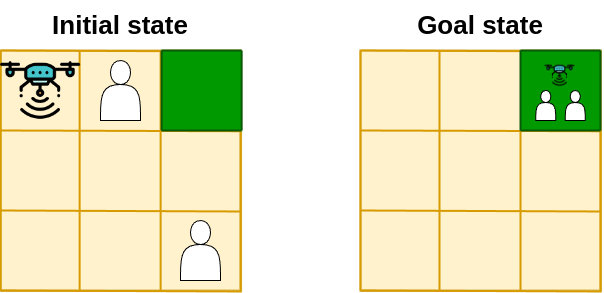
\includegraphics[width=0.55\textwidth]{assets/problem-1-basic.drawio.png}
    \caption{Case 1: Basic}
    \label{fig:initial-state}
\end{figure}

% \begin{figure}[ht]
%     \centering
%     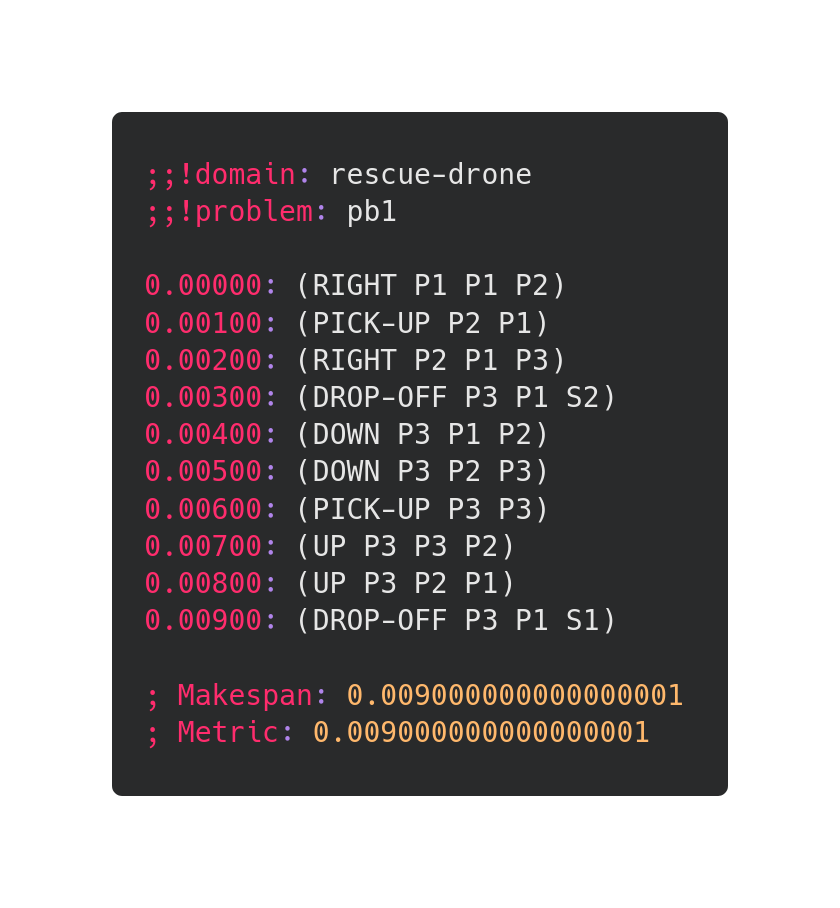
\includegraphics[width=0.55\textwidth]{assets/solution_coordinates/problem-1-plan.png}
%     \vspace{-1cm}
%     \caption{Solution Plan for Case 1: Basic}
%     \label{fig:solution-plan}
% \end{figure}
\FloatBarrier

\subsection{Case 2: Basic with Obstacles}

Subsequently, we incorporate an additional complexity into the model: the presence of obstacles. This scenario replicates the conditions of Case 1, utilizing a small grid and a number of individuals that can be accommodated within the safe zone. However, an obstacle is strategically positioned in the direct path between one of the individuals and the safe zone. This setup is designed to rigorously assess the drone's navigational algorithms and its ability to effectively circumvent obstacles.

\begin{figure}[ht]
    \centering
    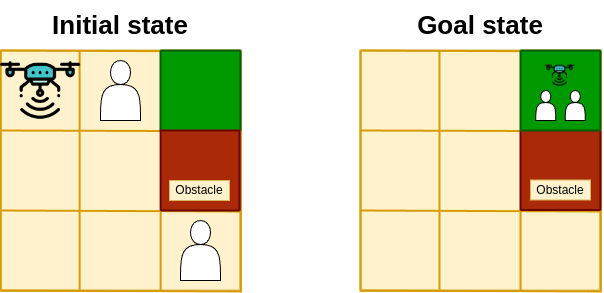
\includegraphics[width=0.55\textwidth]{assets/problem-2-basic-obstacle.drawio.png}
    \caption{Case 2: Basic with Obstacles}
    \label{fig:initial-state-obstacles}
\end{figure}

% \begin{figure}[ht]
%     \centering
%     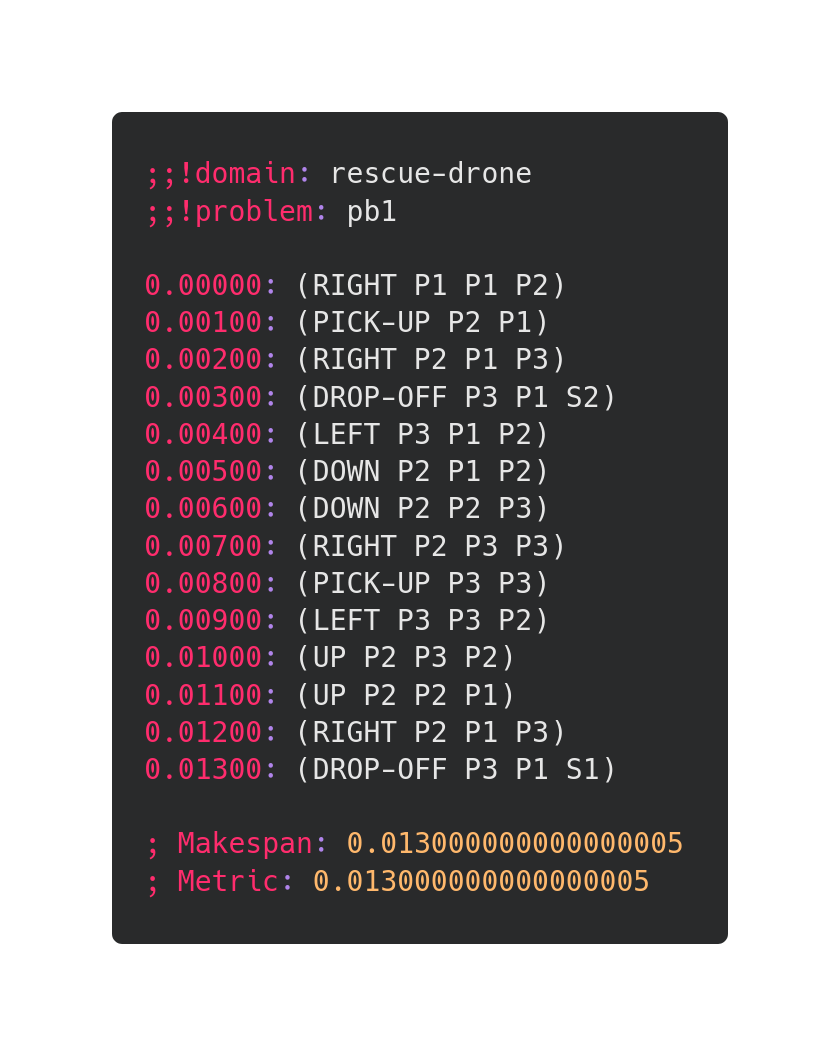
\includegraphics[width=0.55\textwidth]{assets/solution_coordinates/problem-2-plan.png}
%     \vspace{-1cm}
%     \caption{Solution Plan for Case 2: Basic with Obstacles}
%     \label{fig:solution-plan-obstacles}
% \end{figure}
\FloatBarrier

\subsection{Case 3: Overcrowded}

For the next case, we examine another of the features of the model: the capacity of the safe zone. In order to do this, we again utilize a simple layout with a small grid and no obstacles, but in this case, we introduce one more person to rescue, which makes the total number of people bigger than the safe zone capacity. The goal of this test case is to study whether the “spots” feature of the safe zone works as expected.

\begin{figure}[ht]
    \centering
    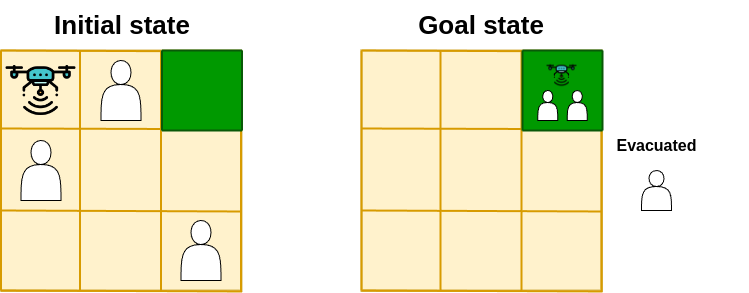
\includegraphics[width=0.55\textwidth]{assets/problem-3-overcrowded.drawio.png}
    \caption{Case 3: Overcrowded}
    \label{fig:initial-state-overcrowded}
\end{figure}

% \begin{figure}[ht]
%     \centering
%     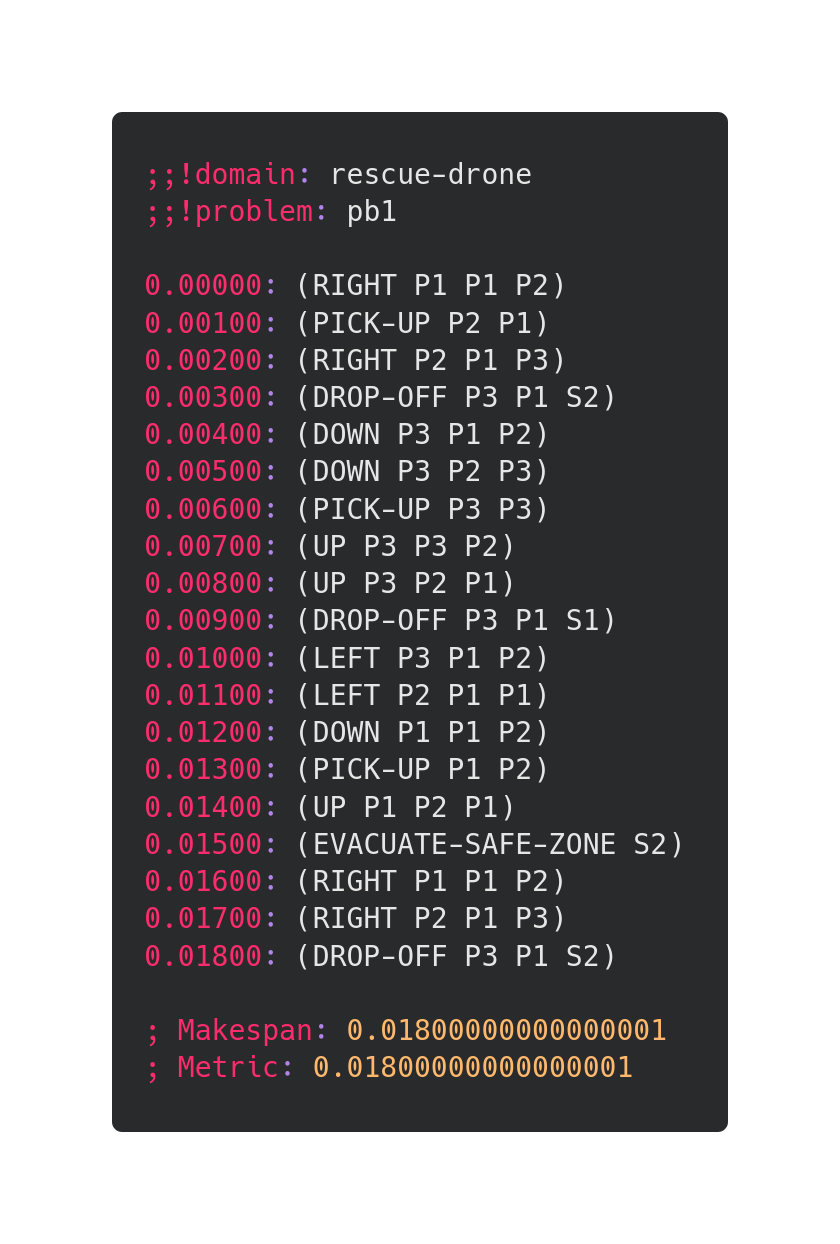
\includegraphics[width=0.55\textwidth]{assets/solution_coordinates/problem-3-plan.png}
%     \vspace{-1cm}
%     \caption{Solution Plan for Case 3: Overcrowded}
%     \label{fig:solution-plan-overcrowded}
% \end{figure}
\FloatBarrier

\subsection{Case 4: Default (PDF example)}

For case 4, we evaluate the default scenario provided as an example in the assignment. This configuration involves rescuing three individuals and navigating around three obstacles within a \(4 \times 4\) grid. This test case is designed to assess nearly all aspects of the model's functionality within a slightly larger grid than previous scenarios.

\begin{figure}[ht]
    \centering
    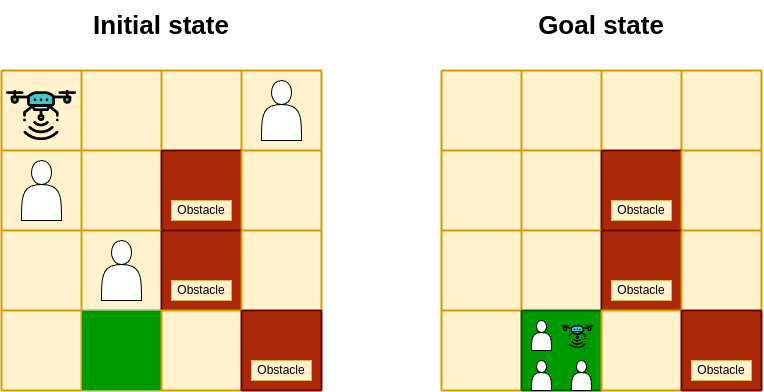
\includegraphics[width=0.55\textwidth]{assets/problem-4-pdf-example.drawio.png}
    \caption{Case 4: Default (PDF example)}
    \label{fig:initial-state-default}
\end{figure}

% \begin{figure}[ht]
%     \centering
%     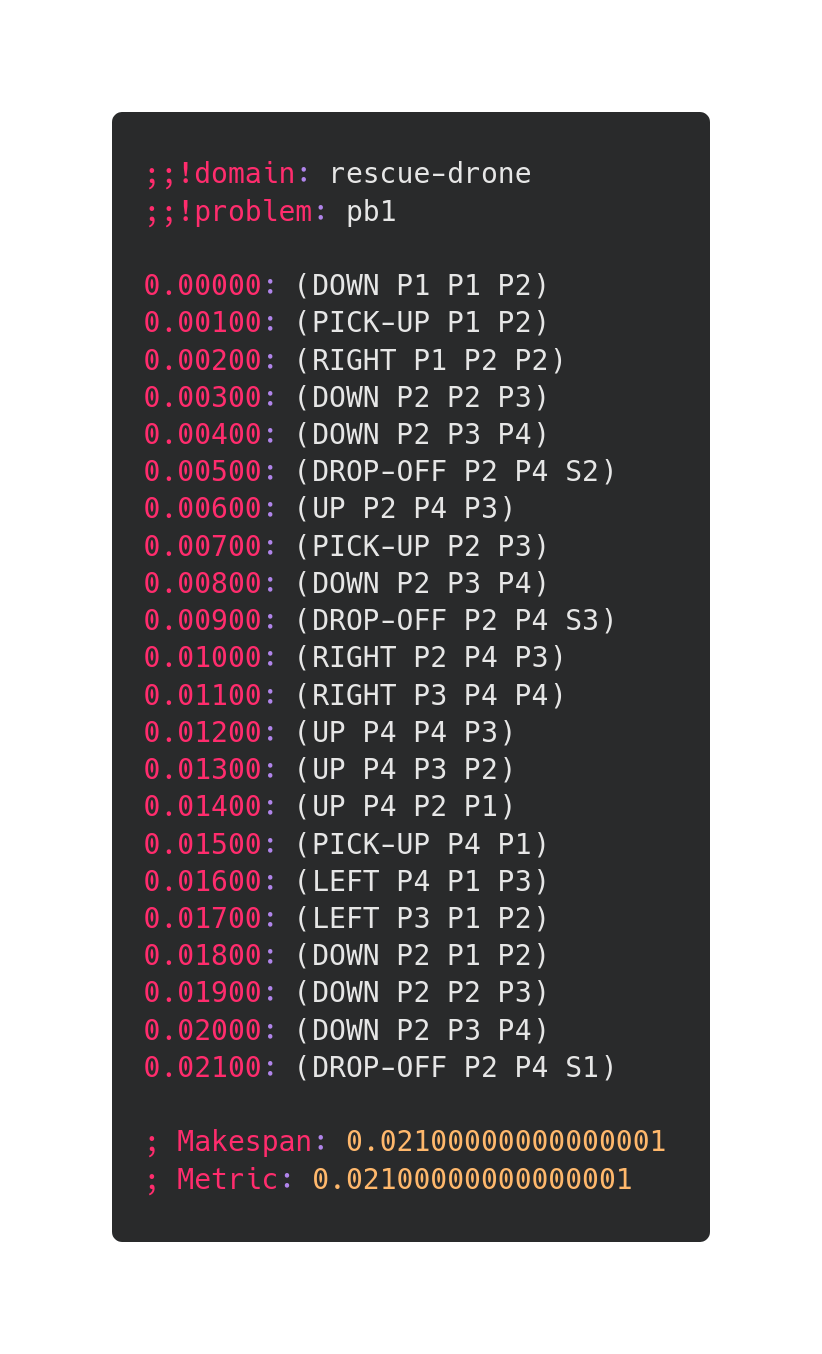
\includegraphics[width=0.55\textwidth]{assets/solution_coordinates/problem-4-plan.png}
%     \vspace{-1cm}
%     \caption{Solution Plan for Case 4: Default}
%     \label{fig:solution-plan-default}
% \end{figure}
\FloatBarrier

\subsection{Case 5: Bigger Grid}

We proceed to conduct a test on a larger grid, specifically a \(5 \times 5\) configuration. This scenario includes five obstacles and six individuals requiring rescue, resulting in a situation where the number of people exceeds the available spots in the safe zone. This comprehensive test case is designed to evaluate all functionalities of the model within a single scenario.

\begin{figure}[ht]
    \centering
    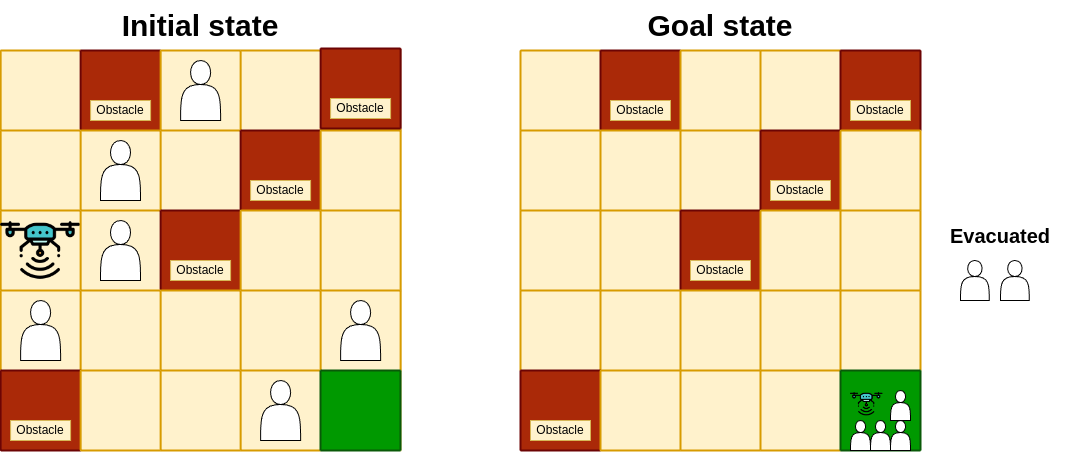
\includegraphics[width=0.55\textwidth]{assets/problem-5-big.drawio.png}
    \caption{Case 5: Bigger Grid}
    \label{fig:initial-state-bigger-grid}
\end{figure}

% \begin{figure}[ht]
%     \centering
%     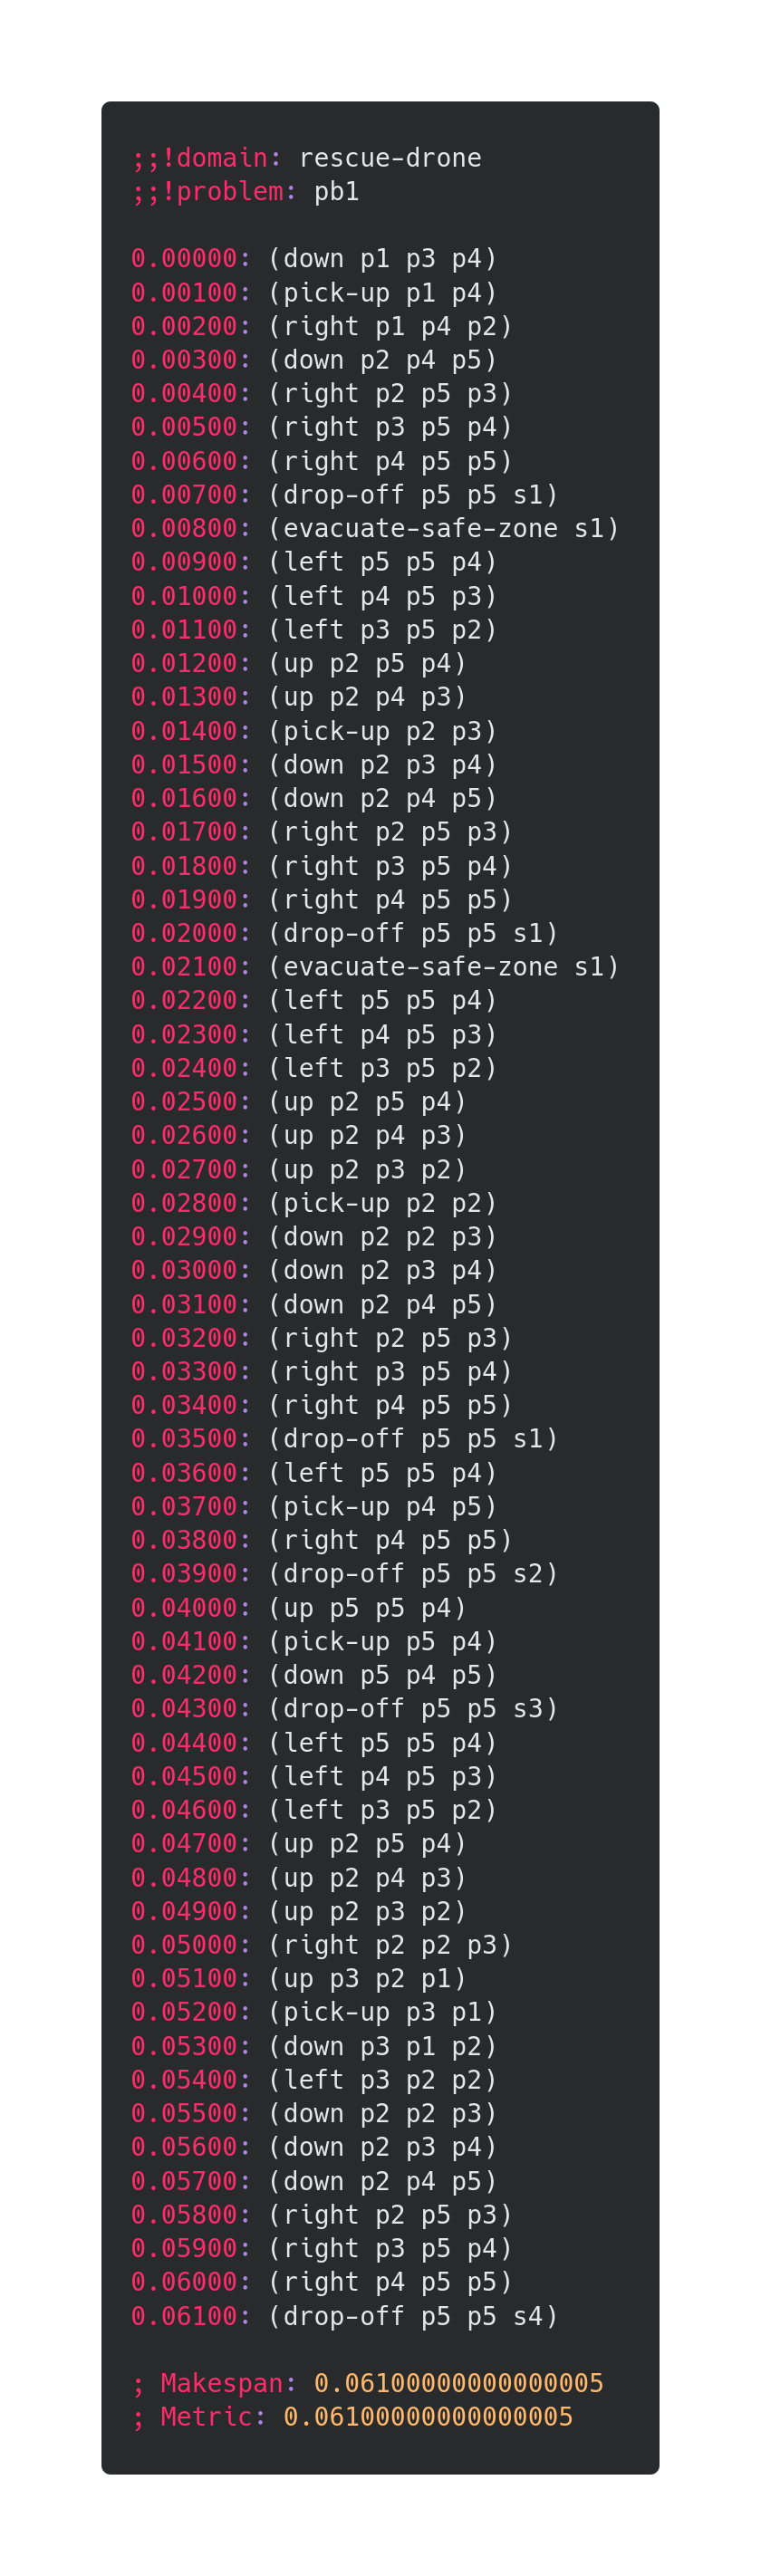
\includegraphics[width=0.55\textwidth]{assets/solution_coordinates/problem-5-plan.png}
%     \vspace{-1cm}
%     \caption{Solution Plan for Case 5: Bigger Grid}
%     \label{fig:solution-plan-bigger-grid}
% \end{figure}
\FloatBarrier

\subsection{Case 6: Maze}

With this test case, we aim to again display all of the functionalities of the model, but this time in a neat and visual scenario that simulates a maze.

\begin{figure}[ht]
    \centering
    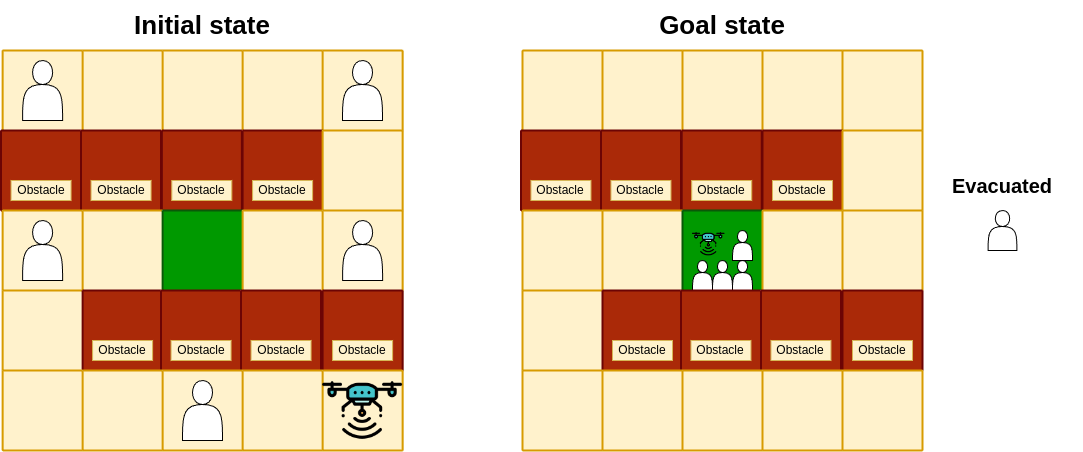
\includegraphics[width=0.55\textwidth]{assets/problem-6-maze.drawio.png} % Increased width
    \caption{Case 6: Maze}
    \label{fig:initial-state-maze}
\end{figure}

% \begin{figure}[ht]
%     \centering
%     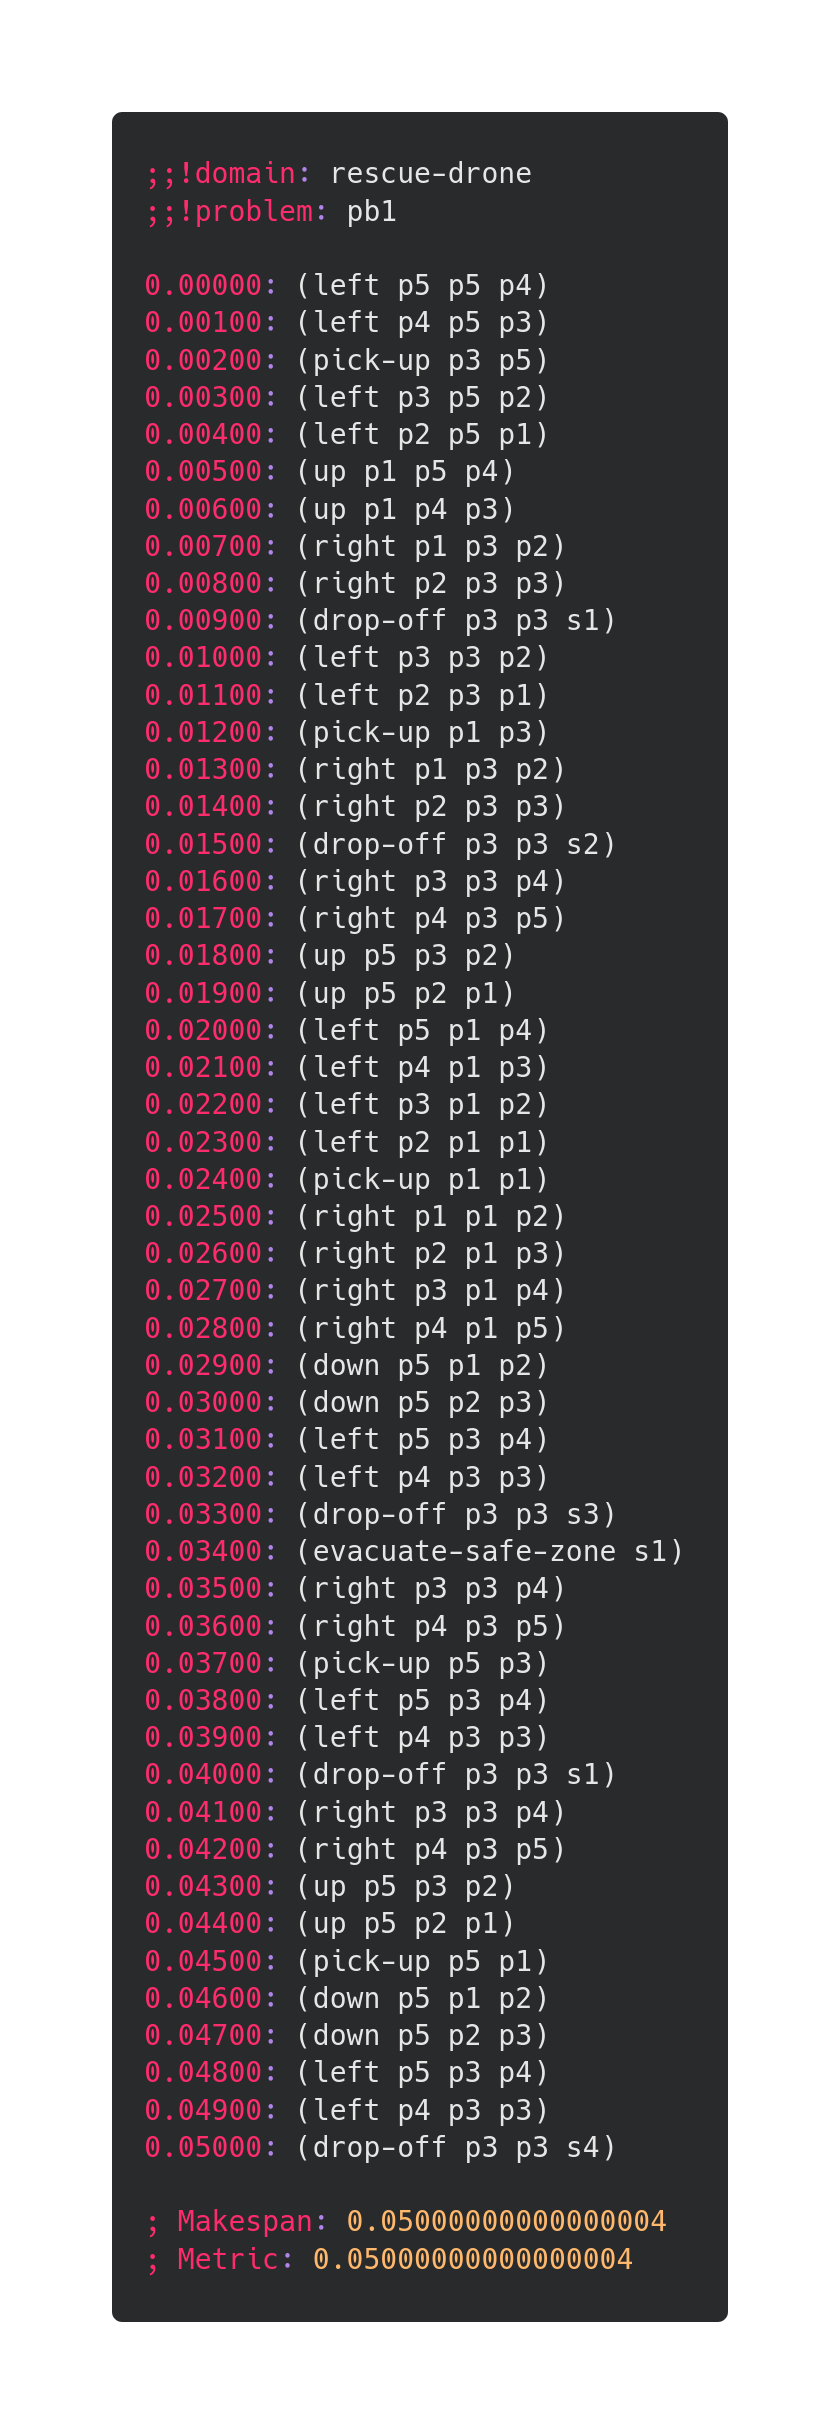
\includegraphics[width=0.55\textwidth]{assets/solution_coordinates/problem-6-plan.png} % Increased width
%     \vspace{-1cm}
%     \caption{Solution Plan for Case 6: Maze}
%     \label{fig:solution-plan-maze}
% \end{figure}
\FloatBarrier

\subsection{Case 7: Impossible}

Finally, as a way to showcase the limits and restrictions of the model, we introduce a test case which is unsolvable. In this layout, the safe zone is fully surrounded by obstacles, and the only possible way to access it might be by moving diagonally, which is currently not an allowed type of movement.

\begin{figure}[ht]
    \centering
    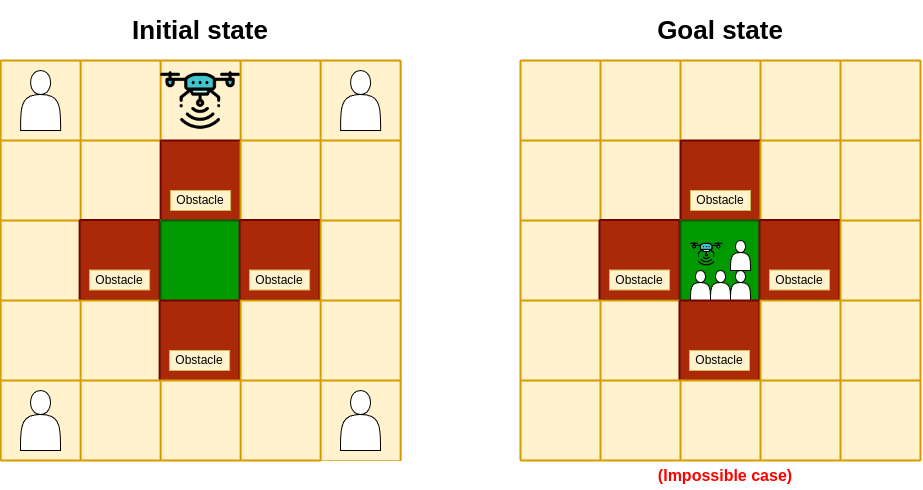
\includegraphics[width=0.55\textwidth]{assets/problem-7-impossible.drawio.png} % Increased width
    \caption{Case 7: Impossible}
    \label{fig:initial-state-impossible}
\end{figure}
\FloatBarrier

\section{Conclusion}


\end{document}